\documentclass[aspectratio=169,kulak,t]{kulakbeamer} % handout

\usepackage[dutch]{babel}
\usepackage[T1]{fontenc}
\usefonttheme[onlymath]{serif}

\title[Beamer]{Smart City}
\subtitle{Presentatie}
\author[Groep 6]{Groep 6} 
\institute[Kulak]{KU Leuven Kulak}
\date{Academiejaar 2020 -- 2021}

\AtBeginSection[]{\only<beamer>{\addtocounter{framenumber}{-1}
		\begin{outlineframe}\frametitle{Overzicht}
			\tableofcontents[currentsection,hideallsubsections]
\end{outlineframe}}}


\begin{document}
	
	\begin{titleframe}
		\titlepage
	\end{titleframe}
	
	\begin{outlineframe}[Overzicht]
		\tableofcontents
	\end{outlineframe}

\section{Aanpak}


\subsection{Planning}
\begin{frame}
	\frametitle{Planning}
	\begin{itemize}
		\item Onderdelen vergelijken
		\begin{itemize}
			\item Budget in rekening houden
			\item Stuklijst
		\end{itemize}
		\item Technisch
		\begin{itemize}
			\item 3D-modellen
			\item Technische tekeningen
		\end{itemize}
		\item Praktisch
		\begin{itemize}
			\item Assemblage
			\item Testen
			\item Implementatie
		\end{itemize}
	\end{itemize}
	
\end{frame}

\subsection{Onderdelen}

\begin{frame}
	\frametitle{Microcontroller \& chassis}
	\begin{columns}
		\column{.5\textwidth}
		\begin{figure}
			\centering
			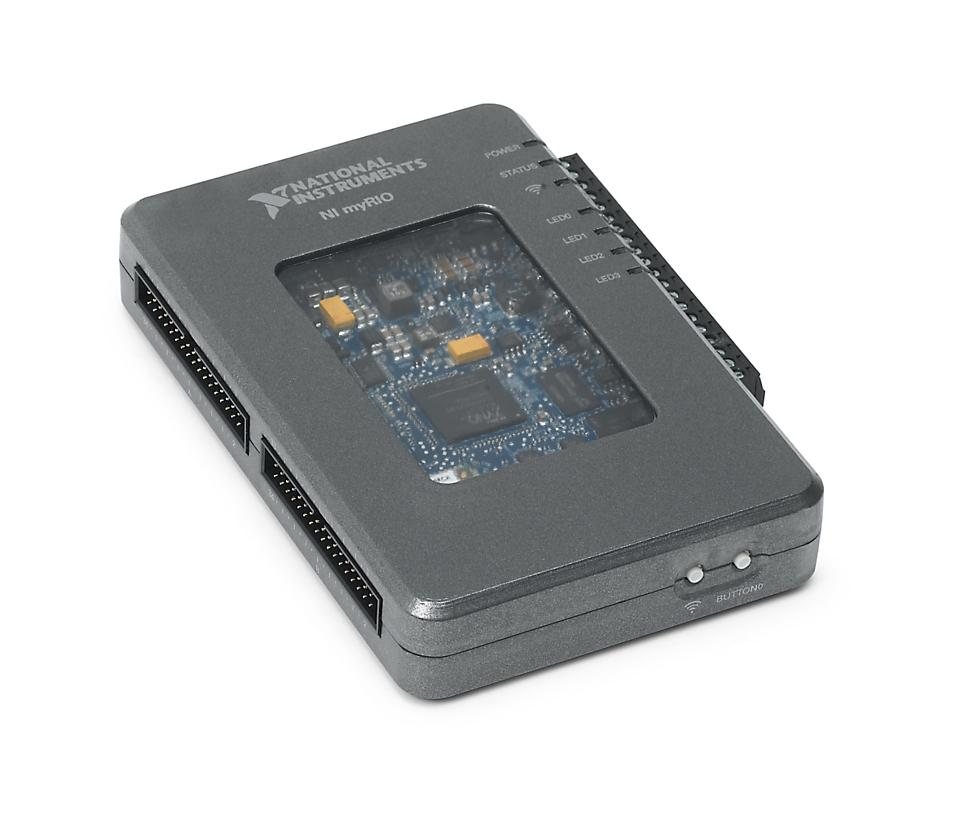
\includegraphics[width=.7\textwidth]{NI-myrio}
			\caption{NI MyRio}
		\end{figure}
		\column{.5\textwidth}
		\begin{figure}
			\centering
			
\includegraphics[width=.7\textwidth]{chassis}
			\caption{Chassis}
		\end{figure}
		
	\end{columns}
	
\end{frame}

\begin{frame}
	\frametitle{Wielen \& ball caster}
	\begin{columns}
		\column{.5\textwidth}
		\begin{figure}
			\centering
			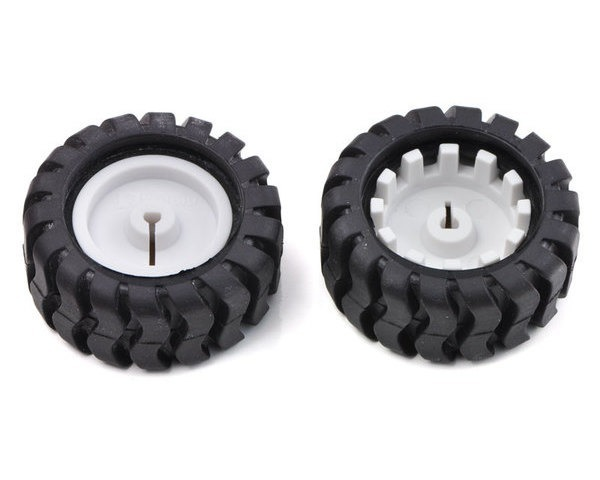
\includegraphics[width=.7\textwidth]{wielen}
			\caption{Wiel 42x19mm}
		\end{figure}
		\column{.5\textwidth}
		\begin{figure}
			\centering
			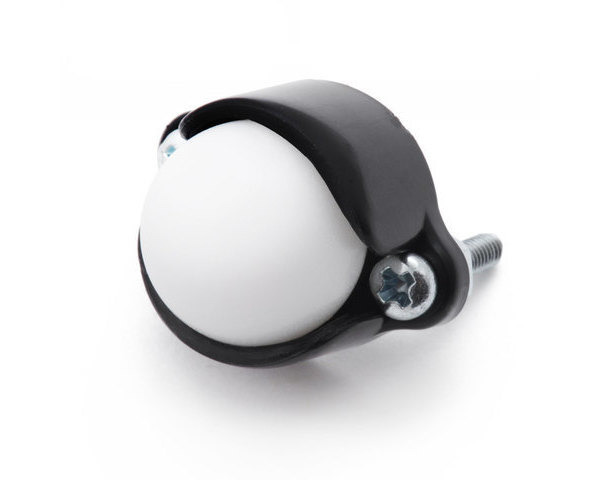
\includegraphics[width=.7\textwidth]{ballcaster}
			\caption{Ball Caster}
		\end{figure}
	\end{columns}
	
\end{frame}

\begin{frame}
	\frametitle{Sensoren}
	\begin{columns}
		\column{.3\textwidth}
		\begin{figure}
			\centering
			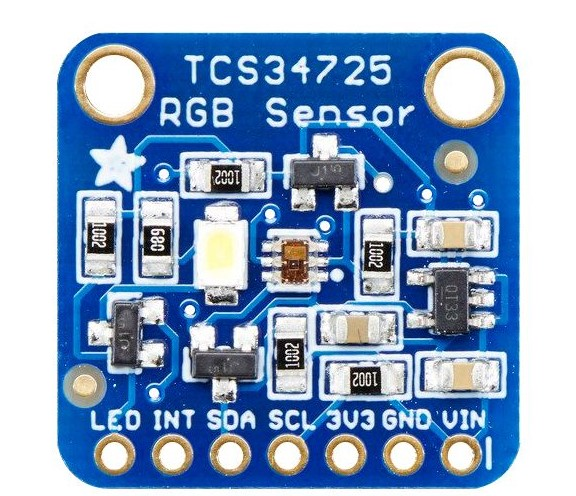
\includegraphics[width=.7\textwidth]{kleurensensor}
			\caption{Kleurensensor}
		\end{figure}
		\column{.3\textwidth}
		\begin{figure}
			\centering
			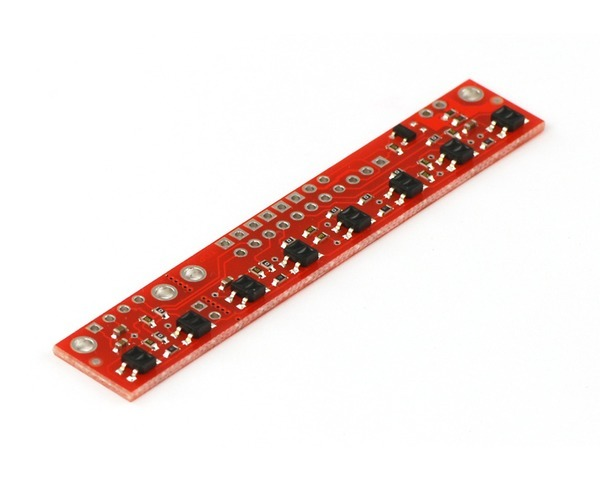
\includegraphics[width=.8\textwidth]{reflectiesensor}
			\caption{Analoge reflectiesensor}
		\end{figure}
		\column{.3\textwidth}
		\begin{figure}
			\centering
			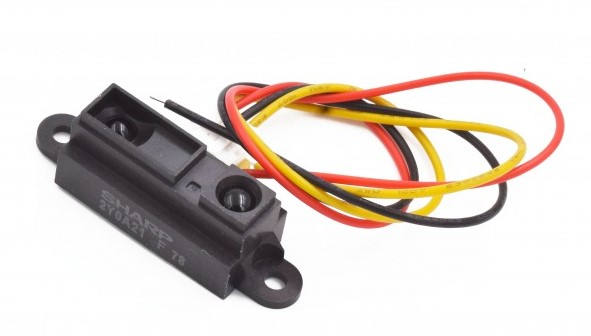
\includegraphics[width=.9\textwidth]{afstandssensor}
			\caption{Analoge afstandssensor}
		\end{figure}
	\end{columns}


\end{frame}

\begin{frame}
	\frametitle{Gear Motor}
	\begin{columns}
		\column{.5\textwidth}
		\begin{figure}
			\centering
			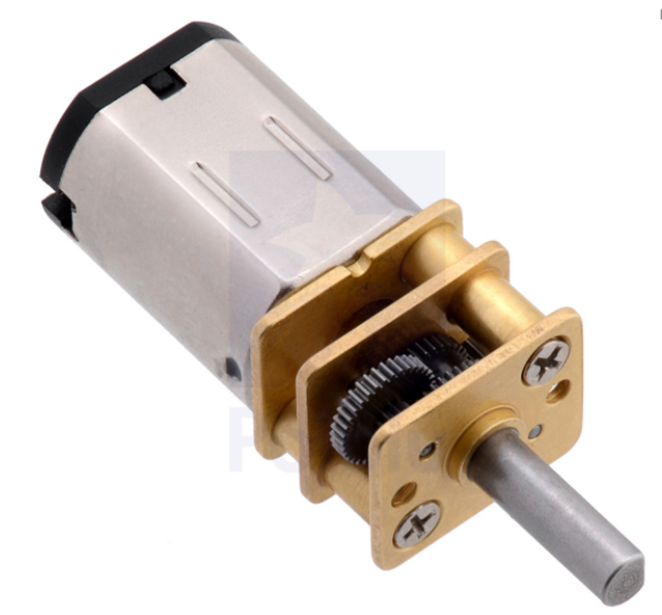
\includegraphics[width=.6\textwidth]{gear}
			\caption{Micro Metal Gear Motor 50:1 HP}
		\end{figure}
		\column{.5\textwidth}
		\begin{figure}
			\centering
			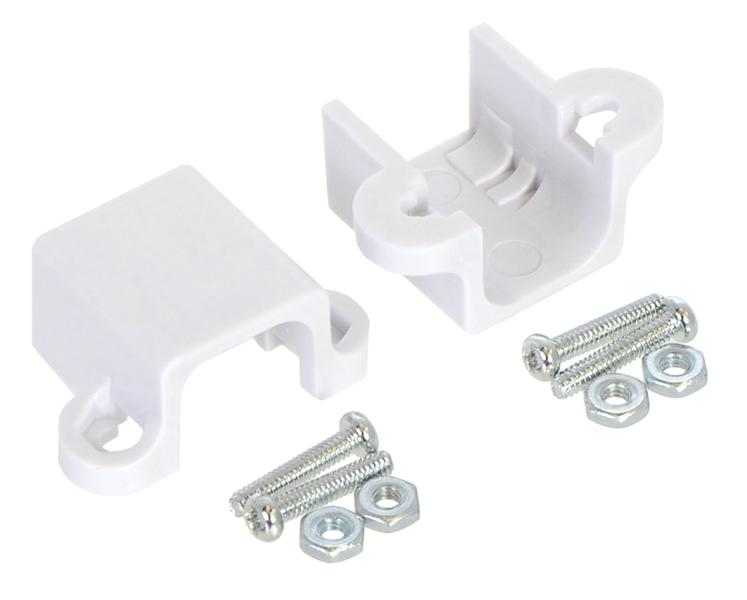
\includegraphics[width=.7\textwidth]{beugel}
			\caption{Motorbeugel}
		\end{figure}
	\end{columns}
	
\end{frame}



\subsection{Prijsbesteding}
\begin{frame}
	\frametitle{Prijsbesteding}
	\begin{itemize}
		\item Budget: 3500 eenheden
		\item Bieding: 1350 eenheden
		\item Uitgave aan onderdelen: 1615 eenheden
	\end{itemize}
\end{frame}
\end{document}